\documentclass[11pt]{article}

\usepackage{acl}
\usepackage{times}
\usepackage{latexsym}
\usepackage[T1]{fontenc}
\usepackage[utf8]{inputenc}
\usepackage{microtype}
\usepackage{inconsolata}
\usepackage{graphicx}
\usepackage{booktabs}
\usepackage{amsfonts}
\usepackage{nicefrac}
\usepackage{xcolor}
\usepackage{subfig}
\usepackage{url}
\usepackage{fancyhdr}

% Figure path for the standalone ACL project folder
\graphicspath{{figures/}}

\setlength\titlebox{6.5cm}

\pagestyle{fancy}
\fancyhf{}
\fancyfoot[C]{\footnotesize Github Link: \url{https://github.com/rohan-crypto/Text_Analytics_Team33_Task3}}
\renewcommand{\headrulewidth}{0pt}
\renewcommand{\footrulewidth}{0pt}


\title{How Has AI Research Changed? 

A Comparative Corpus Analysis of ArXiv Abstracts from 2007 to 2021}

\author{%
\begin{tabular}{ccc}
\normalfont Nithya Dharshini Uthayasankar & \normalfont Rohan Bhardwaj & \normalfont Clarence Zhen Jin Tan \\
\normalfont 2789572 & \normalfont 2827658 & \normalfont 2828537 \\
\end{tabular}
\\[0.8em]
\begin{tabular}{cc}
\normalfont Lingjuan Shu & \normalfont Taojie Chen \\
\normalfont 2739919 & \normalfont el25631, 2764623 \\
\end{tabular}
\\[0.8em]
\normalfont Department of Data Science \\
\normalfont University of Bristol
}

\begin{document}
\maketitle
\thispagestyle{fancy}
\pagestyle{fancy}

\begin{abstract}
The rapid evolution of research in artificial intelligence, machine learning, and natural language processing over the past two decades makes their scientific literature an important source for monitoring their conceptual and methodological changes over time. However, their changes in research focus, communication and terminologies remain ambiguous. Whether using different analytical methods results in different changes has also not been much explored. This corpus analysis addresses that critical gap by dividing 27,121 ArXiv abstracts published between 2007 and 2021 into three five-year periods and comparing them. A two-axis approach is adopted, comparing text representation methods like TF-IDF, SBERT and LDA, against period-comparison methods Textrank, Logistic Regression classification and Framing heatmap using SBERT. The greatest change is identified between 2012-2016 and 2017-2021, uniform across all five methods with a noticeable shift from probabilistic and logic-based topics to neural and language-based approaches, as identified by LDA. The logistic regression classifier trained on TF-IDF features outperforms TextRank in identifying terminologies with respect to a period. Meanwhile, the framing heatmap produced by SBERT confirms decline from research focused on theory to benchmark-based research. These results are aligned with the shift in AI research after 2017 due to the emergence of the Transformer, BERT, and GPT-3. Different methods show different aspects of change, suggesting that corpus-level temporal analysis requires experimentation with multiple methods. As the literature grows, such analysis enables efficient monitoring and tracking of the scientific evolution over time.

\textbf{Keywords:} ArXiv abstracts, corpus analysis, temporal drift, semantic embeddings, topic modelling
\end{abstract}

\section{Introduction}
Research in machine learning (ML), natural language processing(NLP) and artificial intelligence (AI) have been changing rapidly in recent years due to frequent changes in the methods, terminology and research focus. Hence, new theories, methods and vocabulary were extended when certain topics became prominent within a few years.
This makes AI-related scientific literature a useful source for analysis especially with scientific abstracts since it would summarise the research papers. Besides, abstracts would highlight their overall contributions which means analysing abstracts can help the academia to know where the research attention and scientific problems have been changed over time.
To efficiently analyse the scientific abstracts, this project has employed comparative corpus analysis so that changes in vocabulary, dominant methods, and research contributions can be efficiently examined over time. Firstly, datasets related to ML, NLP and AI have been obtained from the HuggingFace arXiv abstracts dataset which contains useful metadata like abstracts and publication years \cite{huggingfaceGfissorearxivabstracts2021Datasets}.
The corpus contains 27121 abstracts and has been carried for preprocessing to better compare the changes in research across the different periods, whereby the corpus has been divided into three five-year periods since research in artificial intelligence only surged especially after 2010 \cite{cao2026decreasing}.
The period 2007-2011 contains 1,268 abstracts , the period 2012-2016 contains 5,542 abstracts, and the period 2017-2021 contains 20311 abstracts. This grouping allows the early, middle, and more recent stages of development in research related to AI to be compared.
The Initial analysis of the dataset reveals frequencies of terms associated with AI increases over time. For instance, as shown in Figure~\ref{fig:lda_topics} it reveals that the abstracts with terms associated with optimisation, probabilistic modelling and statistical approaches in pre-2017 while post-2017 shows an increase in abstracts with terms associated with neural-based, language-based, and learning-based approaches. Hence, this analysis concludes how the research areas in AI have been shifted over the years and how the abstracts in later periods have reflected the rise of deep learning and language-based methods \cite{feng2024evolution}. 
The aim of this project would be to use abstracts as evidence to determine how research related to AI has changed the topic focus and communication over time. The analysis investigates how research attention, scientific problems and terminologies shifted across the three periods. Instead of treating change based on increase or decrease in the term frequency, the project determines if the abstracts have shown significant change in terms of methods, topics and contributions being emphasised by the researchers. Hence, shifts in research topics and scientific problems can be compared across the period to show how AI, ML and NLP have evolved from 2007 to 2021.
To address the aim, this project compares several text analytics approaches that provide different findings from the same corpus. For instance, prominent and terms in a specific period would be identified through vocabulary-based methods while abstracts from different periods would be examined through semantic and topic-based methods to determine if research focus has been different across the periods. The findings would then be evaluated and compared to assess whether the different methods would reveal insights with similar or different patterns of change. Overall, this project seeks to answer two research questions which is how did the topic focus and communication relating to AI, ML and NLP change between 2007 and 2021, and how do the different text analytics methods affect the insights derived from the same corpus?

\section{Methods}
\label{sec:methods}

\subsection{Pipeline Overview and Baseline}
\begin{figure}[ht]
    \centering
    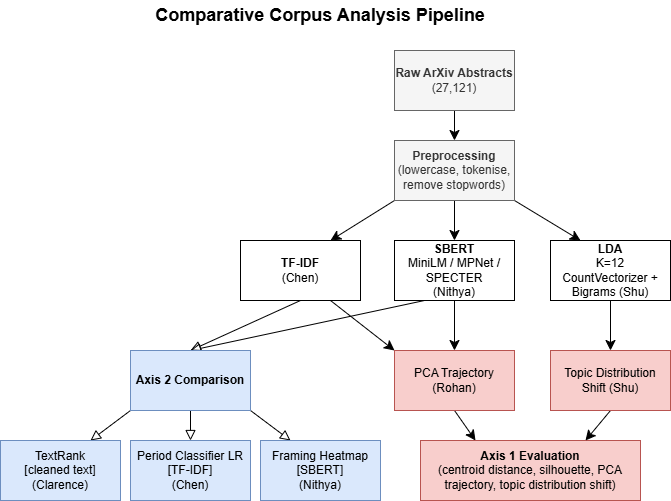
\includegraphics[width=\linewidth]{figures/Comparative_Corpus_Analysis_Pipeline.png}
    \caption{End-to-end analysis pipeline. Text representations feed into two axes of experimentation: representation type (Axis~1) and period-comparison method (Axis~2).}
    \label{fig:pipeline}
\end{figure}

Our corpus comes from the \textsc{ArXiv} dataset \cite{arxiv_dataset}, which includes 27{,}121 abstracts of studies on artificial intelligence, machine learning, and natural language processing. We divided these abstracts into three non-overlapping groups based on when they were published: 2007-2011, 2012-2016, and 2017-2021. And these groups had 1{,}268, 5{,}542 and 20{,}311 abstracts respectively. This clearly shows how quickly research is growing in this field, with more and more studies being published every year.

\paragraph{Preprocessing:}
We preprocessed and cleaned the abstracts before representation. We made them lowercase, tokenised them into individual words and removed common stop-words like "the" and "and" because they do not add much meaning. We also got rid of the punctuation marks. For TF-IDF, we only looked at the 5{,}000 most important features using \texttt{TfidfVectorizer} from \texttt{sklearn}, with both unigram and bigram (n $\in \{1,2\}$). We did not apply stemming because the SBERT models, which we are using, are good at handling morphological variation. Instead, we worked directly with the original text to understand what each sentence means.

\subsection{Axes of Experimentation}
We have set up our investigation to focus on two main axes that are independent of each other, and each one targets a different aspect of how we analyse things.

\subsection{Axis~1: Text Representation Methods}
\textbf{Axis~1 - Text Representation:} \textit{How does our way of text representation influence the insights that we gain about changes over time?}
We look at three different ways to do this: TF-IDF, SBERT, and LDA. Each one is unique because it focuses on different aspects of the text. TF-IDF focuses on how often certain vocabulary appears on the surface, SBERT considers the context and meaning of words, and LDA explores the latent topics that are present. By comparing these methods using the same corpus and evaluation metrics, we can see how the choice of representation affects our understanding. This comparison helps us understand the strengths and weaknesses of each method, which is important for drawing accurate conclusions about change over time.

\subsubsection{TF-IDF (Chen)}
TF-IDF represents each abstract as a sparse weighted vector made up of a 5{,}000-token vocabulary. Term weights show a term's importance in a document compared to the entire corpus. Common words get lower weights, while unique ones receive higher weights. To get period-level representations, we average all abstract vectors for each time window to create a centroid. Then we measure inter-period drift using the cosine distance between successive centroids.
\textbf{Hypothesis:} The hypothesis is that TF-IDF will be good at picking up vocabulary shifts on the surface level. Like when new trendy terms come into fashion, such as "transformer" or "pre-trained". This will, in turn, produce large centroid displacements. However, it will not be great at understanding when the same concept is being talked about, but with different terminology, across different time periods. TF-IDF will think it's a completely new topic. This can lead to major changes in the grouping of the topics, even if the underlying idea is still the same.

\subsubsection{SBERT (Nithya)}
We test three pre-trained sentence-transformer models while we increase the domain specialisation. They include \textbf{MiniLM} (\texttt{all-MiniLM-L6-v2})~\cite{reimers-gurevych-2019-sentence}, a lightweight encoder for general tasks, \textbf{MPNet} (\texttt{all-mpnet-base-v2}), a large encoder for general tasks, and \textbf{SPECTER}~\cite{specter2020cohan}, a model pre-trained on scientific citations. Each abstract is represented as a 384 or 768-dimensional dense vector. The period centroids and cosine distances between them are calculated exactly as in TF-IDF. These SBERT embeddings are also used in Axis 2. They are used to calculate cosine distance between each period's centroid and 6 predefined sentences of specific framing archetypes such as "state-of-the-art", "theoretical", "real-world application", "new dataset", "scaling up" and "interpretability". This gives us a heatmap showing the research framing trend.
\textbf{Hypothesis} SBERT will perform better at detecting semantic drift as compared to TF-IDF because dense embeddings contain semantic information rather than exact tokens. But there will be a less directly interpretable embedding space. We will know \emph{how much} the field changed, but not exactly \emph{what} changed. Domain-specific SPECTER embeddings should result in denser within-period clustering than general-purpose models.

\subsubsection{LDA Topic Model (Shu)}
The corpus is fit to a Latent Dirichlet Allocation~\cite{blei2003latent} (LDA) model with K=12 topics, which were determined by perplexity analysis. Each abstract is represented as a 12-dimensional topic-proportion vector. Topic distribution for each time period is the average topic vector for all abstracts in the time period. The drift between time periods is calculated by using the Euclidean distance between successive period centroids. This distance is computed from the fully pairwise distance matrix (\texttt{lda\_period\_distances.npy}). To measure how the three time periods cluster, we calculate the average silhouette score on the topic-proportion vectors. With this, LDA can be directly compared with TF-IDF and SBERT on both of the evaluation metrics used in Axis 1.
\textbf{Hypothesis} We think that using LDA will help us find hidden thematic patterns in our data that we cannot see with TF-IDF and SBERT. This could show us which big areas of research, like neural generation or probabilistic inference, are getting more or less popular over time. But the way LDA works can be a bit unpredictable, as it may vary with K, so the results might change depending on our hyperparameter choice. Smaller absolute centroid distances and a near-zero silhouette score are expected, since the dimensionality of topic-proportion space ($K{=}12$) will be low relative to the dimensionality of topic space for TF-IDF ($V{=}5{,}000$) and SBERT (384-768 dimensions). This will lead documents to contain most topics at varying proportions, rather than being clustered by distinct topics.

\subsubsection{PCA Temporal Trajectory (Rohan)}
To make it easier to visually compare different representations, Principal Component Analysis (PCA) is applied to each one. This includes the TF-IDF matrix and the SBERT embedding matrices, like MiniLM, MPNet, and SPECTER. Each of these is then simplified into its first two principal components, which show the maximum variance. These simplified versions are then plotted on a 2D graph, with colours used to show which time period each point belongs to. The centroids of each period are connected with arrows to show a \emph{temporal trajectory}. This helps us evaluate the first axis. If the periods are clearly separated on the graph, it's easier to interpret what is going on, no matter the distance between the points. The resulting trajectories are shown in Figure~\ref{fig:pca_trajectory} in Section~\ref{sec:evaluation}.

\subsection{Axis~2: Period-Comparison Methods}
\textbf{Axis~2 - Period-Comparison Method:} \textit{What comparison method shape and affect the specificity and interpretability of the results?}
Even with a fixed representation, different comparison strategies may give different qualitative signals. To see that, we compare an inductive, frequency-based approach (TextRank) with a discriminative, supervised approach (a period classifier). Then we enhance the analysis by using SBERT to compare sentences and identify their underlying themes.

\subsubsection{TextRank Keyword Extraction (Clarence)}
TextRank~\cite{mihalcea-tarau-2004-textrank} is a way to figure out what's important in a document. It is an unsupervised graph-based algorithm. It looks at how words are used together, models them as a graph and gives them a PageRank-style score. We apply TextRank to all the abstracts from a certain time window, and then aggregate the results to get a ranked list of key phrases. It helps us make a list of the most important phrases for each period. This method is \emph{inductive}. It looks at each period on its own, without comparing it to other periods, which gives us a sense of what was important during that time, and what phrases were being used a lot.
\textbf{Hypothesis} Our idea is that TextRank can find domain-appropriate words that were used frequently in a certain time period, like "neural network" from 2017 to 2021. But it has a drawback that it does not compare different time periods, so it will also find words that are common in \emph{all} time periods, like "machine learning". This means it will miss words that became more or less popular over time, even if the change was big.

\subsubsection{Period Classifier (Chen)}
\label{sec:classifier}
We trained a multinomial logistic regression classifier on the TF-IDF matrix that helps us predict which of three periods an abstract belongs to, based on the words it contains. We train it using 80\% of the abstracts and then test it on the remaining 20\% to see how well it works. The good thing about this approach is that the TF-IDF features are easy to interpret because they are based on the actual words in the abstracts. The classifier gives more weight to words that are unique to a particular period, rather than just words that appear frequently in that period. This helps us identify the words that really distinguish one period from another, which is exactly what we need to detect changes over time.
\textbf{Hypothesis} When trained with a contrastive objective, the classifier will produce signals that are more focused and more time period specific as compared to TextRank. For instance, the words "pre-trained", "graph neural", and "federated learning" should emerge as good positive discriminators of the time span 2017-2021. On the other hand, older paradigms such as "logic programming" and "influence diagram" will emerge as good negative discriminators for the same period. Results across all three periods are compared in Figure~\ref{fig:axis2_all}.

The framing heatmap, developed by Nithya for SBERT, offers a unique perspective that builds on the keyword methods. Instead of focusing on the topics being discussed, it looks at how research is presented and structured, revealing changes in the way ideas are framed over time. For instance, it shows how theoretical approaches have become less prominent, while practical applications have gained more attention across different periods. The heatmap is shown in Figure~\ref{fig:framing_heatmap}.

\subsection{Summary of Design Choices}

Table~\ref{tab:methods_summary} summarises all methods, their contributors, and their role in the pipeline.

\begin{table}[ht]
\centering
\caption{Methods summary. CosDist = cosine distance; EuclDist = Euclidean distance.}
\label{tab:methods_summary}
\resizebox{\linewidth}{!}{%
\begin{tabular}{llll}
\toprule
\textbf{Method} & \textbf{Contributor} & \textbf{Axis} & \textbf{Distance Metric} \\
\midrule
TF-IDF (bigram, $V{=}5000$)      & Chen     & 1 and 2 & CosDist \\
SBERT MiniLM                      & Nithya   & 1 and 2 & CosDist \\
SBERT MPNet                       & Nithya   & 1 and 2 & CosDist \\
SBERT SPECTER                     & Nithya   & 1 and 2 & CosDist \\
LDA ($K{=}12$)                    & Shu      & 1      & EuclDist \\
PCA Trajectory (TF-IDF \& SBERT) & Rohan    & 1      & Visual / centroid \\
TextRank Keyword Extraction       & Clarence & 2      & Frequency rank \\
Logistic Regression Classifier    & Chen     & 2      & Coefficient magnitude \\
SBERT Framing Heatmap             & Nithya   & 2      & CosDist to archetype \\
\bottomrule
\end{tabular}}
\end{table}

\section{Experimental Evaluation}
\label{sec:evaluation}

\subsection{Performance Metrics}
We evaluated each method on three related performance metrics, because no definitive answer exists as the correct temporal change for an unsupervised corpus analysis.

\paragraph{Centroid cosine distance:} 
For TF-IDF and SBERT, we compute the cosine distance between centroids in consecutive periods. For LDA we look up in the pre-calculated pairwise distance matrix (\texttt{lda\_centroid\_dist[i][j]}) and extract the Euclidean distance between consecutive period centroids in 12-dimensional topic-proportion space. Larger distance implies more quantifiable change between periods. Since distances are calculated in different representation spaces, the absolute values of distances are not directly comparable between methods.. \emph{Limitation:} The raw value is only comparable between methods of the same type (both TF-IDF), as different embedding spaces will have different geometries. Centroid shift may not represent general drift but may be caused by a single outlying sub-corpus in a single period.

\paragraph{Silhouette score:}
For each abstracted period, the silhouette score~\cite{rousseeuw1987silhouettes} measures how well each abstract fits its own period cluster when compared to the nearest alternative period. Values near $+1$ indicate well-separated clusters and very tight periods, $0$ implies overlapping clusters, and a negative value suggests that the abstract was fit to the incorrect period cluster. \emph{Limitation:} The score may be skewed if the clusters have an imbalance (the corpus is strongly dominated by 2017-2021, $n{=}20{,}311$) and it will score global separation over gradual change.

\paragraph{Interpretability:}
For Axis-2, we compare each pair of abstract terms and qualitatively assess whether the top-ranking terms are period-specific or generic. Higher scores for methods that produce period-specific term suggestions over common words across periods.

\subsection{Experimental Setup}

\paragraph{Dataset splits:}
The 27,121 abstracts are split into three consecutive non-overlapping time periods of 2007-2011 (n=1,268), 2012-2016 (n=5,542) and 2017-2021 (n=20,311). The dates for the period splits were chosen to coincide with well-known milestones in AI/ML research. The start date of the "deep learning wave", defined as when AlexNet achieved significant performance, is 2012; the second time boundary is around the Transformer paper and the introduction of BERT in 2017-2018; and GPT-3, introduced in 2020, falls within the third period. All abstracts were part of unsupervised analyses (TF-IDF centroids, SBERT embeddings, LDA and TextRank). A stratified split into a training set (80\% of data) and a testing set (20\% of data) was performed to preserve the proportion of the periods in the dataset for the period classifier (Section~\ref{sec:classifier}).

\paragraph{Hyperparameters:}
TF-IDF was implemented with unigrams and bigrams up to a maximum of 5,000 terms (\texttt{sklearn} \texttt{TfidfVectorizer}). We used SBERT models as they are without fine-tuning: MiniLM (\texttt{all-MiniLM-L6-v2}) of 384-d, MPNet (\texttt{all-mpnet-base-v2}) of 768-d, and SPECTER~\cite{specter2020cohan} of 768-d. LDA was fit with K=12 topics, which were determined based on held-out perplexity. The logistic regression classifier was fit with an $\ell_2$ penalty using $C=1$ (the default in \texttt{sklearn}). TextRank was run on each document individually using a 4-token co-occurrence window, and document phrase scores were then averaged over all documents for a given time period.

\paragraph{Libraries:}
Text representation methods for \texttt{sklearn}~\cite{sklearn} TF-IDF and LDA; \texttt{sentence-transformers}~\cite{reimers-gurevych-2019-sentence} for SBERT; \texttt{pytextrank} for TextRank. Dimensionality reduction methods: \texttt{sklearn} PCA. Evaluation metrics: \texttt{sklearn} silhouette scorer and \texttt{scipy} for distance metrics.

\subsection{Results}

\subsubsection{Axis~1: Centroid Distance}
Table~\ref{tab:centroid_distances_and_silhouette_score} and Figure~\ref{fig:centroid_bar} report centroid distances between successive periods for all five representations.

\begin{table}[ht]
\centering
\caption{Centroid distances and silhouette scores for all five representations.}
\label{tab:centroid_distances_and_silhouette_score}
\resizebox{\linewidth}{!}{%
\begin{tabular}{lcccc}
\toprule
\textbf{Method} & \textbf{2007--11 $\to$ 2012--16} & \textbf{2012--16 $\to$ 2017--21} & \textbf{Mean shift} & \textbf{Silhouette Score} \\
\midrule
TF-IDF (bigram, $V{=}5000$) & 0.2595 & 0.2889 & 0.2742 & 0.0015 \\
SBERT MiniLM                 & 0.0461 & 0.1221 & 0.0841 & 0.0541 \\
SBERT MPNet                  & 0.0500 & 0.1388 & 0.0944 & 0.0559 \\
SBERT SPECTER                & 0.0055 & 0.0298 & 0.0177 & 0.0172 \\
LDA ($K{=}12$)               & 0.0270 & 0.2733 & 0.1502 & 0.0029 \\
\bottomrule
\end{tabular}}
\end{table}

\begin{figure}[ht]
    \centering
    
\includegraphics[width=\linewidth]{figures/axis1_grouped_bar_chart.png}
    \caption{Centroid distances between consecutive period pairs for all five methods. Blue bars = 2007-2011 to 2012-2016 transition; red bars = 2012-2016 to 2017-2021 transition. Every method records a larger shift in the second transition.}
    \label{fig:centroid_bar}
\end{figure}

There are two recurring features in all 5 of the methods. The first recurring feature is that each method recorded a larger change from 2012-2016 to 2017-2021 than from 2007-2011 to 2012-2016, thus verifying that the rate of change accelerated due to the Transformer (2017), BERT (2018) and GPT-3 (2020). The second recurring feature is that the ranking of mean shift (TF-IDF > LDA > SBERT-MPNet > SBERT-MiniLM > SBERT-SPECTER) represents the various geometric properties of each space, rather than a measure of their sensitivity to real change. TF-IDF's large, sparse 5,000-dimensional vocabulary space amplifies cosine distances, while SBERT's dense embeddings reduce them.
The most remarkable single finding is LDA's near-zero first-transition distance (0.0270) followed by its large second-transition distance (0.2733), a tenfold increase. The topics are largely unchanged from 2007-2011 to 2012-2016, and it is the vocabulary that is altered as captured by TF-IDF due to the deep-learning trend, rather than the thematic domains. However, the change in thematic domains is substantial, since the 2016 Transformer and BERT research rewrote the entire field of NLP.

\begin{figure}[ht]
    \centering
    
\includegraphics[width=\linewidth]{figures/axis1_transition_year_range_comparison.png}
    \caption{Difference in centroid distance between the two transitions (second minus first) for each method. All bars confirm the 2012-2016 to 2017-2021 transition was larger across every representation type. LDA shows the greatest relative difference (+0.2463).}
    \label{fig:transition_diff}
\end{figure}

\subsubsection{Axis~1: Silhouette Scores}

Table~\ref{tab:centroid_distances_and_silhouette_score} and Figure~\ref{fig:silhouette} report overall silhouette scores for all five representations.

\begin{figure}[ht]
    \centering
    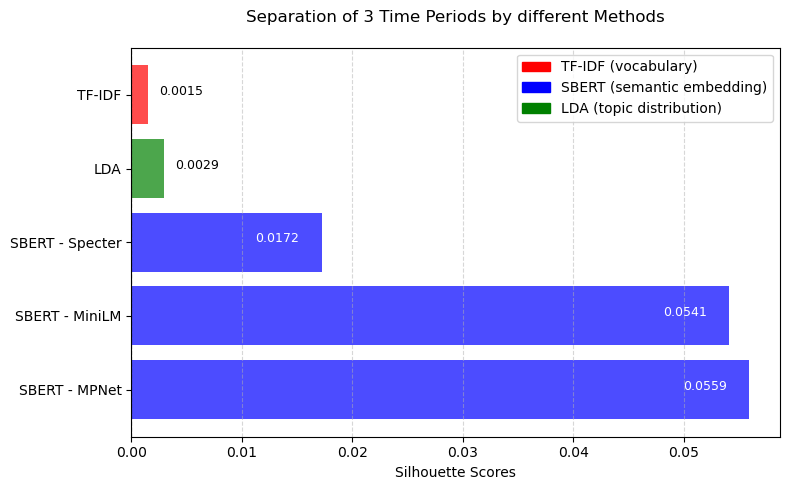
\includegraphics[width=\linewidth]{figures/silhouette_score.png}
    \caption{Silhouette scores for all five representations. Red = TF-IDF (vocabulary-based); blue = SBERT variants (semantic embedding); green = LDA (topic distribution). SBERT MPNet achieves the highest period separability.}
    \label{fig:silhouette}
\end{figure}

All silhouette scores are low, which is expected. The drift in topic over time within abstracts of academic papers is a gradual, not discrete. The late 2016 and early 2017 abstracts deal with similar topics, meaning that no strict boundaries lie between periods.
Significantly, both SBERT MiniLM (0.0541) and MPNet (0.0559) performed much better at separating periods than TF-IDF (0.0015), and this result partially contradicts our hypothesis for Axis-1. TF-IDF was hypothesised to be more sensitive to differences at the period level, yet it was the poorest representation in terms of cluster cohesion. The reason TF-IDF's 5,000-dimensional sparse space is the weakest here is that the between-period variance is still too low, and within-period variance, where every abstract had a unique combination of vocabulary terms, was too high. Due to this reason, its centroids are poor representatives of the distributions for each period.
SPECTER underperformed the other SBERT models (0.0172), unlike what we had predicted. We thought that SPECTER's domain-specific pre-training would lead to tighter clusters, but SPECTER's citation-network training appears to prioritise proximity at the paper-level over coherence at the period level. The silhouette score for LDA (0.0029) indicates that the topic proportions are naturally continuous and shared across periods, and thus do not result in geometrically separable temporal clusters even with the thematic shift.

\subsubsection{Axis~1: PCA Temporal Trajectory}

\begin{figure}[ht]
    \centering
    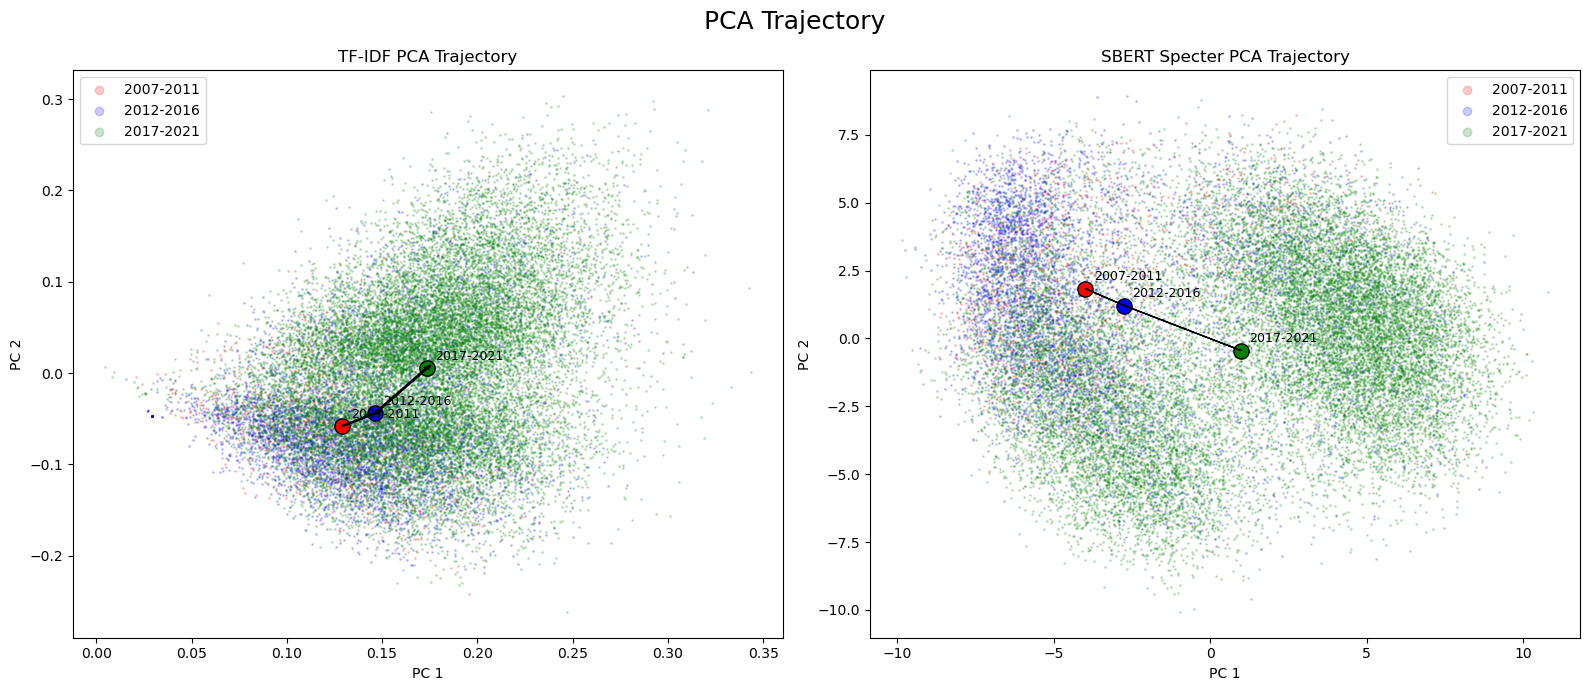
\includegraphics[width=\linewidth]{figures/PCA_trajectory.png}
    \caption{PCA trajectory plots for TF-IDF (left) and SBERT-SPECTER (right). Each point is an individual abstract, colour-coded by period. Larger markers are period centroids; arrows show the direction of temporal drift. The TF-IDF centroid displacement along PC~1 is visibly larger than in SBERT-SPECTER space.}
    \label{fig:pca_trajectory}
\end{figure}

Both views show a consistent drift as the period centroids move consistently from 2007-2011 through 2012-2016 and to 2017-2021. This suggests that the drift is real and not noise. TF-IDF shows more variation along PC-1, which we think is because modern vocabulary around deep-learning fields is largely replacing classical AI vocabulary. SBERT-SPECTER, on the other hand, appears less "spread out". We see that, even as vocabulary changes, closely related fields stay relatively close to each other. We believe this is consistent with SBERT being focused on capturing \emph{how much} the field changed, and not \emph{what} changed.
The large amount of overlap between individual clouds in both spaces confirms our low silhouette score. We are unable to accurately recover the period membership from the abstracts themselves. So, the drift is apparent at the distributional level.

\subsubsection{Axis~1: LDA Topic Distribution}

\begin{figure}[ht]
    \centering
    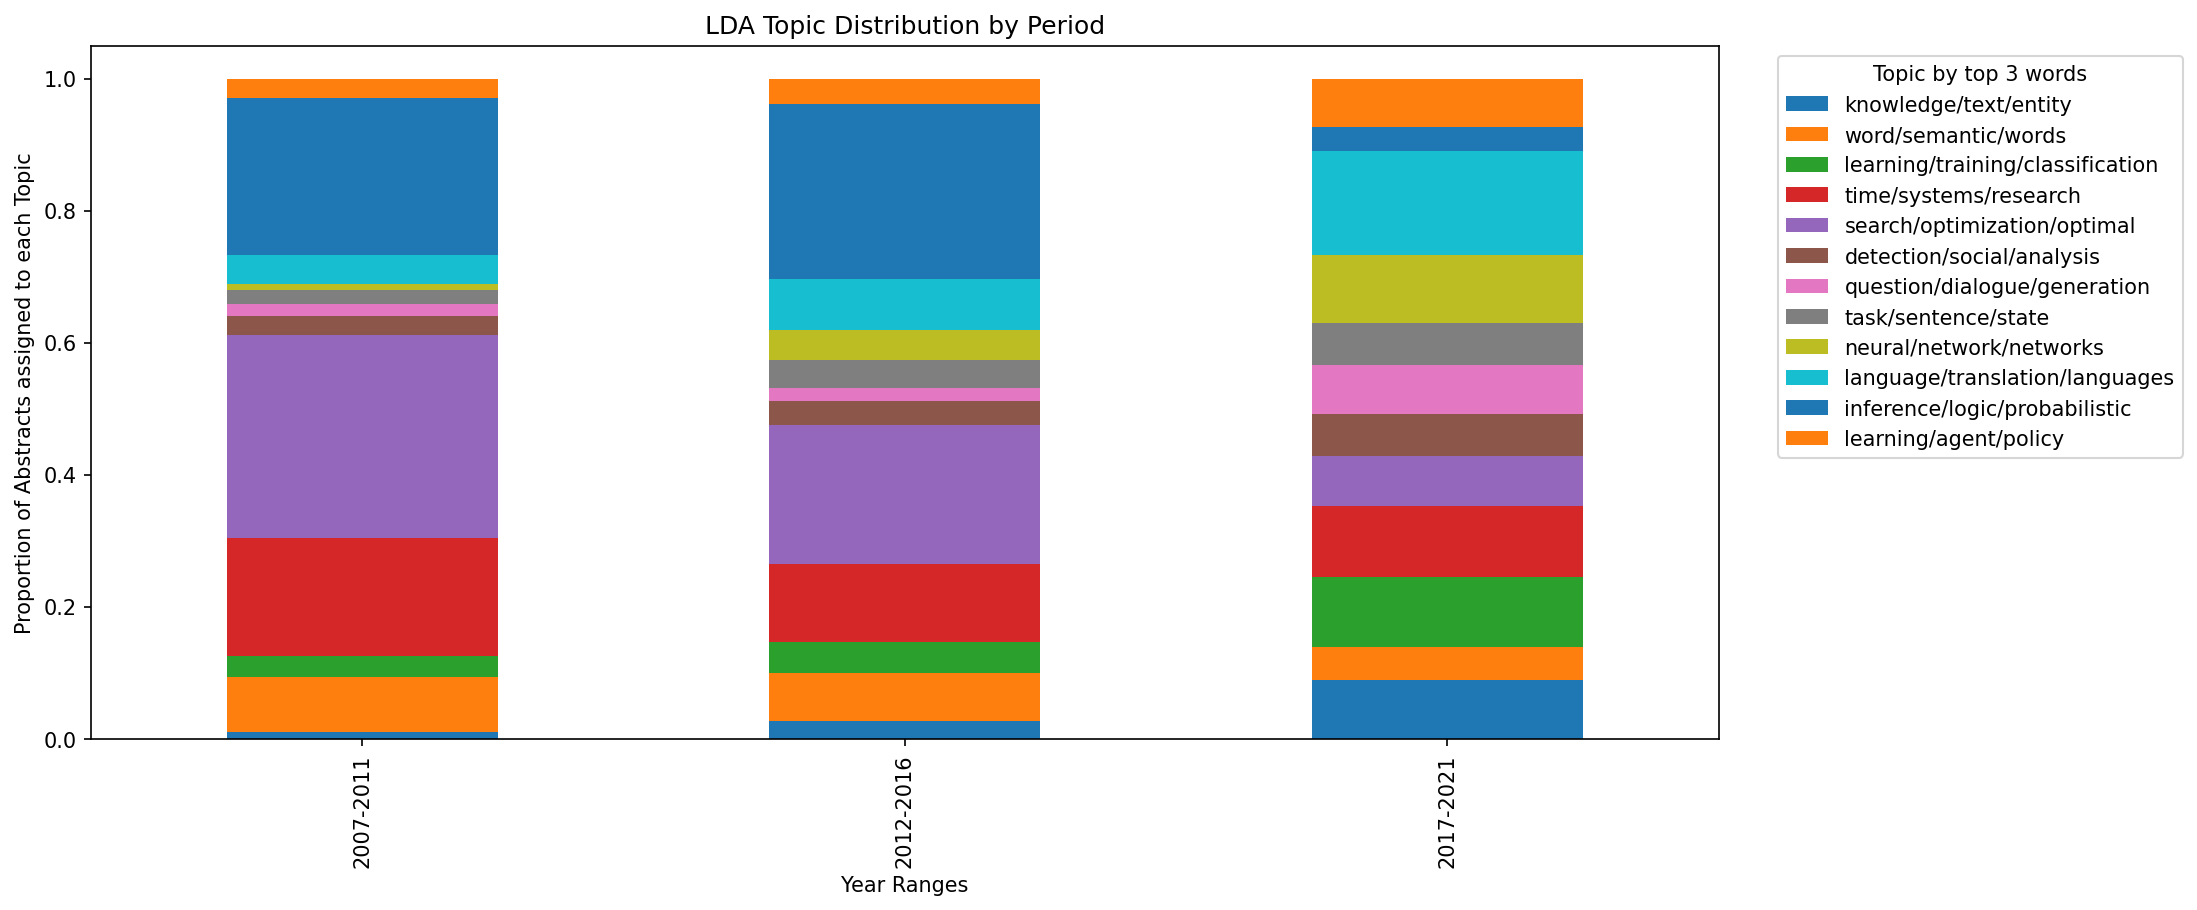
\includegraphics[width=\linewidth]{figures/axis1_lda_topic_distribution.png}
    \caption{Stacked bar chart of LDA topic proportions per period. Each colour represents one of the 12 topics, labelled by its three most probable words. The shift from 2012-2016 to 2017-2021 is the dominant transition.}
    \label{fig:lda_topics}
\end{figure}

\begin{figure}[ht]
    \centering
    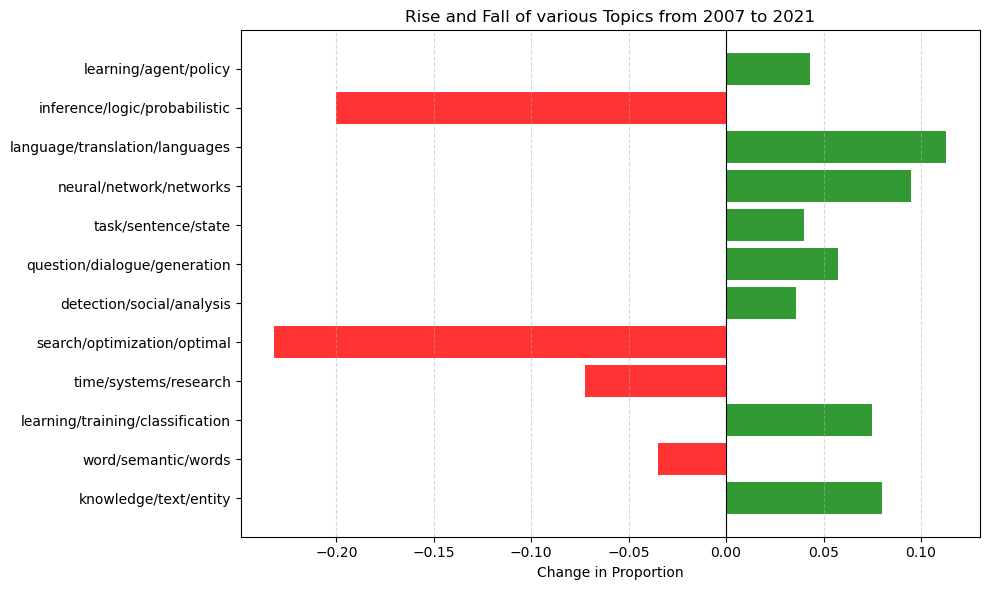
\includegraphics[width=\linewidth]{figures/LDA_topics_shift.png}
    \caption{Net change in LDA topic proportion from 2007-2011 to 2017-2021. Green bars = rising topics; red bars = declining topics. T4 (search/optimisation/optimal) and 
    T10 (inference/logic/probabilistic) show the largest declines; T9 (language/translation/languages) and T8 (neural/network/networks) show the largest rises.}
    \label{fig:lda_change}
\end{figure}

The LDA topic model produces the strongest qualitative description of \emph{what} changed. The topics Figure~\ref{fig:lda_topics} of search/optimisation/optimal (T4) and inference/logic/probabilistic (T10), which dominated 2007--2011 largely disappeared by 2017-2021 (shown in Figure \ref{fig:lda_change}). This directly shows the decline of traditional AI technologies - constraint satisfaction, logic programming, and Bayesian networks, in favour of an end-to-end neural approach. The most prominent changes are the emergence of the neural/network/networks topic (T8), \\ language/translation/languages topic (T9), and question/dialogue/generation topic (T6). T9's increased prominence is quite evident as it was driven by neural machine translation (2016) and the emergence of BERT (2018) and GPT-3 (2020) during or just prior to the 2017-2021 time period. These transitions in topic distribution are invisible to both TF-IDF and SBERT centroid analysis and highlight the unique benefit of LDA, as it identified \emph{what} changed rather than just \emph{how much} changed.

\subsubsection{Axis~2: TextRank vs.\ Period Classifier}

\begin{figure}[ht]
    \centering
    \subfloat[2007--2011]{%
        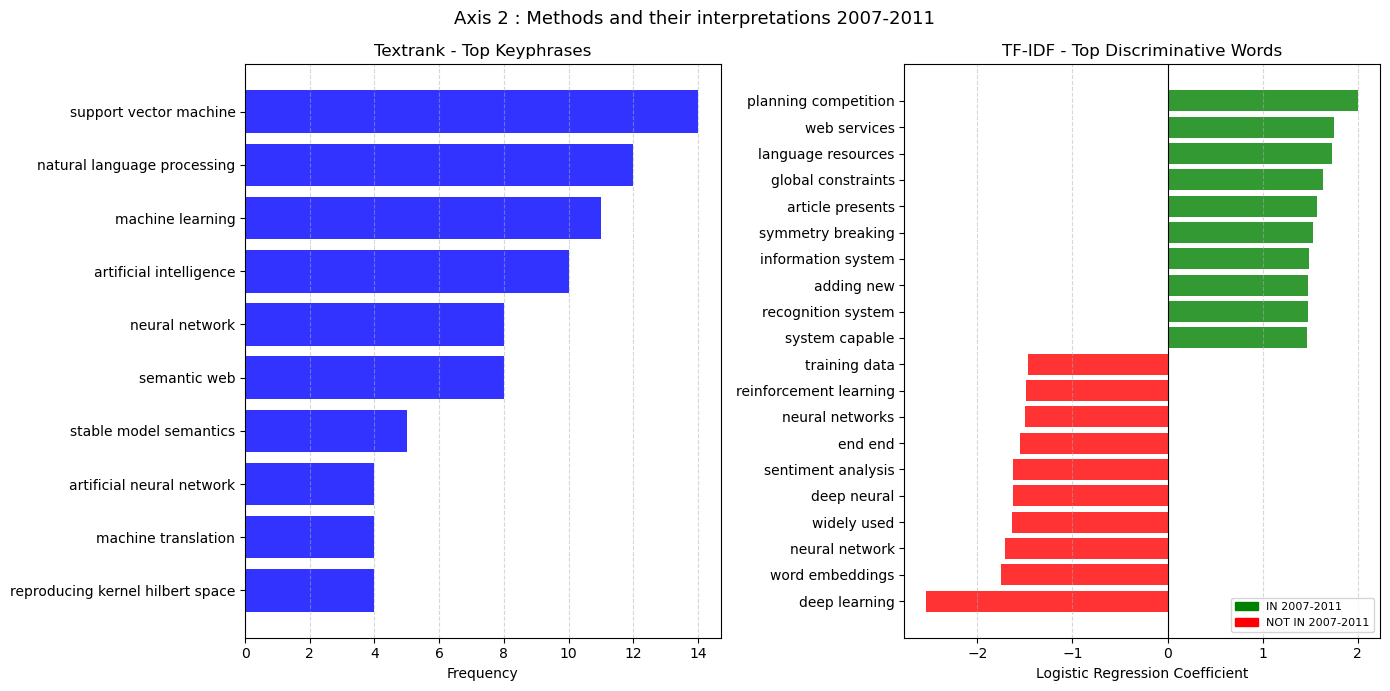
\includegraphics[width=0.95\linewidth]{figures/Axis2_comparison1.png}
        \label{fig:axis2_2007}}\\[4pt]
    \subfloat[2012--2016]{%
        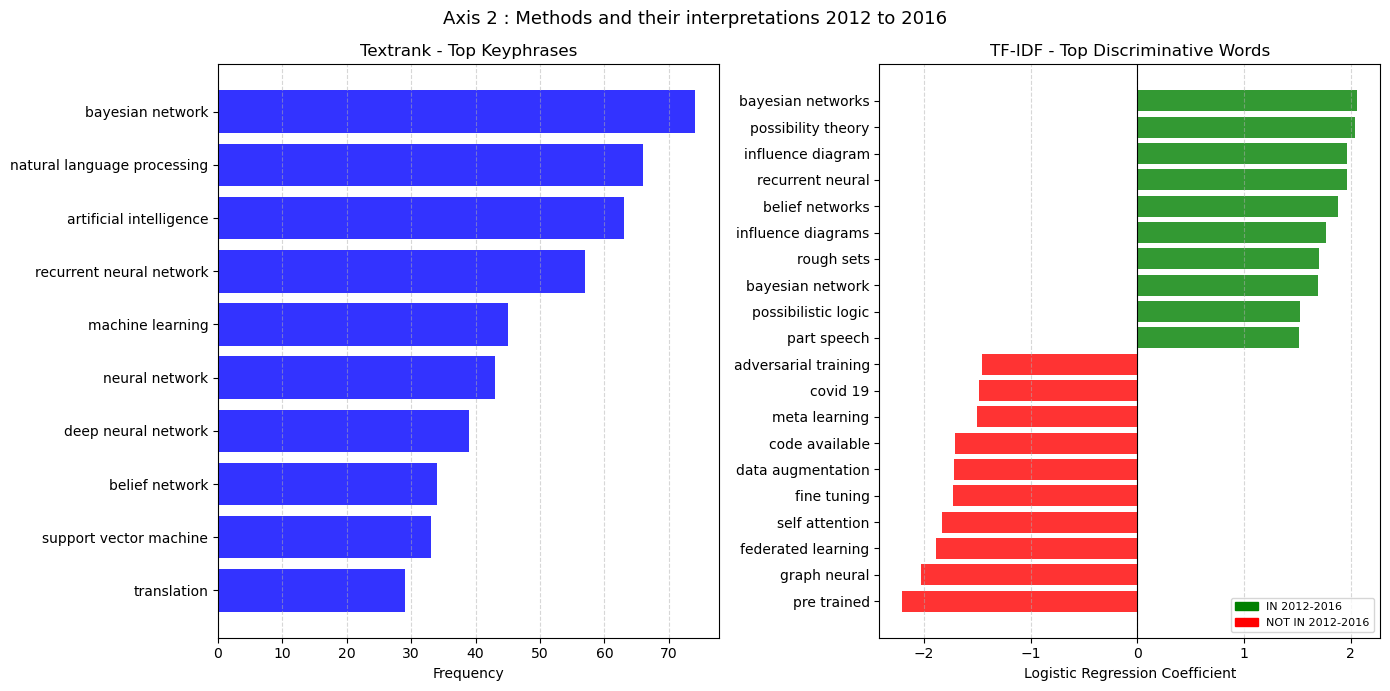
\includegraphics[width=0.95\linewidth]{figures/Axis2_comparison2.png}
        \label{fig:axis2_2012}}\\[4pt]
    \subfloat[2017--2021]{%
        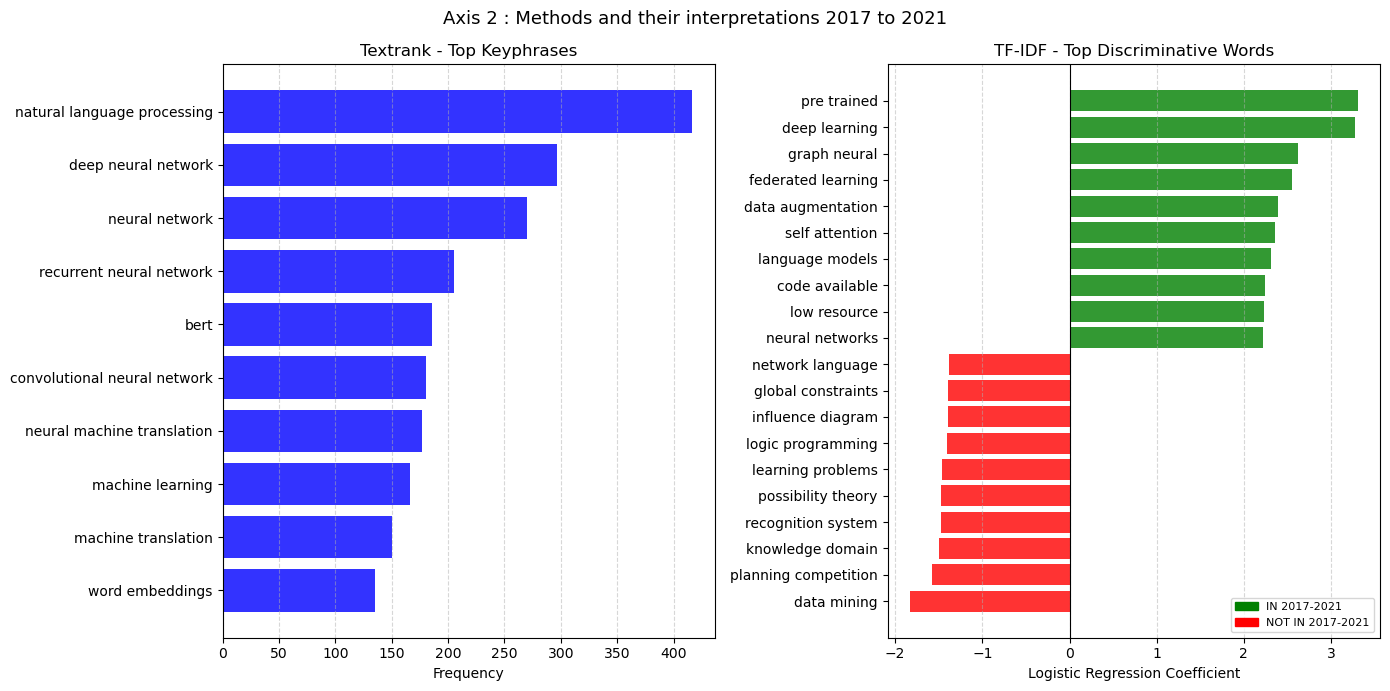
\includegraphics[width=0.95\linewidth]{figures/Axis2_comparison3.png}
        \label{fig:axis2_2017}}
    \caption{Axis~2 comparison for all three periods. Left panel of each subfigure: TextRank top keyphrases. Right panel: logistic regression discriminative coefficients. Green bars = terms strongly predictive \emph{of} that period; red bars = terms strongly predictive \emph{against} it. The contrast between the two methods is most pronounced in 2017--2021, where the classifier uniquely identifies 
    "pre-trained" (+3.30), "graph neural" (+2.62), and "federated learning" (+2.55).}
    \label{fig:axis2_all}
\end{figure}

TextRank identifies keyphrases that occur frequently and represent the domain, but does not differentiate \emph{contrastive} from \emph{prevalent}. The top 2017-2021 TextRank terms include natural language processing (416 times), neural network (270), and machine learning (166), and these appear at the top of the 2012-2016 list too. This supports our Axis-2 hypothesis as well, that TextRank reflects document frequency rather than period-relative frequency, and therefore cannot describe what makes a period distinct.

Using TF-IDF features and training a logistic regression classifier produces discriminative outputs. For 2017-2021, the positive coefficients correspond to pre-trained (+3.30), deep learning (+3.28), graph neural (+2.62), federated learning (+2.55), self-attention (+2.36), and language models (+2.31), which appear prominently with the advent of the Transformer (2017), BERT (2018) and the LLM boom (2020). The negative coefficients reflect the unused classical AI terms, such as data mining (-1.83), logic programming (-1.41), and influence \\ diagram (-1.39). For 2007-2011, the classifier shows planning competition, web services and global constraints to be highly characteristic. These appear nowhere on the TextRank's top 10 for this period. This provides direct evidence for the Axis-2 hypothesis that the model trained to distinguish between periods can find unique features for each period, which simple frequency-based methods like TextRank cannot capture.

\begin{figure}[ht]
    \centering
    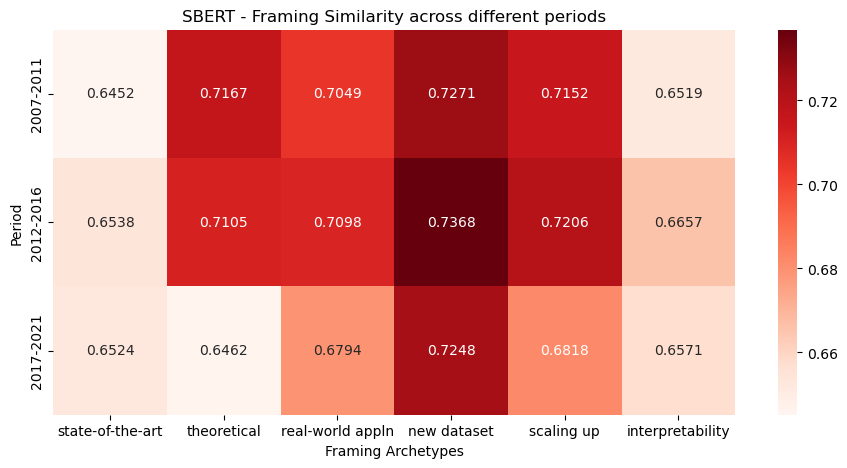
\includegraphics[width=\linewidth]{figures/SBERT_framing_heatmap.png}
    \caption{SBERT framing similarity heatmap. Each cell is the cosine similarity between the period centroid embedding and a hand-crafted framing archetype sentence. The theoretical framing declines most clearly from 2007--2011 (0.717) to 2017--2021 (0.646), while state-of-the-art remains stable, suggesting a shift from theoretically-framed to benchmark-driven research.}
    \label{fig:framing_heatmap}
\end{figure}

Figure~\ref{fig:framing_heatmap} shows that the framing heatmap shows another independent complementary view orthogonal to both keyword methods. Theoretical framing standard decreases monotonically from 0.717 to 0.646 between 2007-2011 and 2017-2021, respectively. Both state-of-the-art and real-world applications are fairly consistent, 0.645-0.652 and 0.705-0.679, respectively. However, the prominent decrease suggests a shift in research towards more empirical, benchmark-oriented work and away from theoretically framed studies, which reflects the leaderboard-based culture in the post-2017 world of NLP and ML. Importantly, this result is derived from purely semantic space and cannot be the result of vocabulary change and thus serves as an independent validation of the classifier.

\subsection{Error Analysis}

\paragraph{Corpus imbalance and TF-IDF:}
The 2017-2021 data is 16 times larger than the 2007-2011 data. Since the centroids of the periods are simple averages and the 2017-2021 period's cohort greatly outnumbers all others, the mean of the period's centroid significantly biases the global TF-IDF mean. Cosine distance involving an early period may therefore be deflated, suggesting it is closer than it appears to another early period or to the global mean. This also aligns with the very low silhouette score for TF-IDF (0.0015). Given that the within-period TF-IDF is an average across vastly different, sparse vocabularies, a period's centroid would make a very poor summary of that period's vocabulary distribution. Thus, it causes high within-period variance. In future work, it might be worth doing an experiment with normalised or resampled centroids that try to account for this imbalance.

\paragraph{Near-zero first transition for LDA:}
The centroid distance of 0.0270 between the 2007-2011 and 2012-2016 periods is unexpectedly small.  A rapid shift in terminology after 2016 would be expected. It may simply be a statistical anomaly driven by a lack of data. The small 2007--2011 cohort (n=$1{,}268$) might be leading to an unstable, possibly noisy centroid that will always converge towards the corpus mean. Or, it is possible that the deep learning revolution simply has not been reflected in the language of abstracts until later on in time, and there is genuinely significant thematic overlap between these two early periods. It is interesting that this cluster of periods also has very low silhouette scores, 0.0029 for LDA and 0.0015 for TF-IDF, supporting the interpretation that many topics overlap between all three periods.

\paragraph{Generic terms for TextRank:}
A number of the top keyphrases, like 'machine learning', 'natural language processing' and 'proposed method', are too generic for the domain of AI abstracts, so they may be more numerous but do not indicate much about change in themes. TextRank might perform better with a contrastive version that down-weights common terms in order to focus on the differences, but that would defeat its unsupervised nature.

\paragraph{Classifier on TF-IDF features only:}
It should be noted that the period classifier was only used on the TF-IDF features. Applying the same discriminative training to SBERT embeddings would help to test whether dense vector representations produce more interpretable or accurate period signals. This can be included in future work.

\paragraph{Variance compression for SBERT framing heatmap:}
All values are within the narrow range of 0.645 - 0.737, so the absolute difference between any two is relatively small, although the direction of change is still very meaningful. This is an inherent limitation of using cosine similarity in dense high-dimensional space. The high dimensionality has resulted in most vectors being nearly equidistant. So, it can be interpreted that, when looking at the heatmap, the relative difference is more meaningful than the absolute difference.

\subsection{Discussion}

\paragraph{Consistency and robustness (Axis-1):}
All five representations have an agreement in regard to direction of drift, which states that 2012-2016 to 2017-2021 is greater than 2007-2011 to 2012-2016, and shows steady improvement. This convergence among fundamentally different methods of sparse frequency counts, dense semantic vectors, and probabilistic topic proportions suggests that the change is real, and not some characteristic of just one method.

\paragraph{Interpretability trade-off (Axis-1):}
TF-IDF offers the highest interpretability because words in the vocabulary explicitly state what has changed. SBERT is highest at understanding meaning as it can still see the topical continuity even when different terminology is used. LDA provides the highest level of structure by revealing underlying themes, but loses a degree of interpretability, given that topics must be identified based on keyword lists. PCA trajectory demonstrates geometric integrity among all three methods, with TF-IDF showing the largest centroid displacement, and SBERT-SPECTER the smallest, clustered centroid.

\paragraph{Specificity vs.\ generality (Axis-2):}
Classifier greatly outperforms TextRank in terms of period specificity. Its terms with the top-weight are specific to a single period, while TextRank includes across-period general terms. Classifier requires labelled periods and a discriminative claim about what \emph{differentiates} periods, whereas TextRank makes a generative claim about what periods are \emph{characterised} by. They are therefore complementary perspectives. The SBERT framing heatmap shows a third, orthogonal angle as it focuses on how things are expressed, instead of topical content, using purely semantic analysis.

\paragraph{Limitations}
The corpus is restricted to English-language ArXiv abstracts, specifically in AI, ML, and NLP, so conclusions may not apply to other fields or other languages. Abstracts may not fully represent the deep methodologies and breadth of the source papers. Temporal windows are too wide, so the intra-period changes might be obscured. For example, 2017-2021 includes the Transformer era as well as the GPT-3 era, both having different characteristics.

\section{Conclusion}
We analysed trends over time in the abstracts of research on AI, ML and NLP across three different periods (2007–2011, 2012–2016, and 2017–2021) to understand the evolution of the field. Using a two-dimensional analytical framework, we compared text representation methods (first axis) with methodological extraction methods (second axis). Finally, our aim is to investigate how these choices of representation and methodology influence perceptions of shifts in academic paradigm.
The results we derived from Axis 1 partially confirmed our initial hypothesis about lexical sensitivity and semantic sensitivity. As predicted, compared to the relatively smooth trajectory seen with SBERT, TF-IDF detected a more significant centroid distance between neighbouring periods (peaking at 0.2889 between 2012–2016 and 2017–2021), demonstrating TF-IDF's high sensitivity to the sudden introduction of new vocabulary. However, the silhouette scores for both TF-IDF (0.0015) and SBERT (0.0559) were close to 0. This suggests that, although the vocabulary changed between periods, individual abstracts showed high diversity during the same period and could not be clearly classified by time. This reflects the continues evolution of concepts rather than distinct ,unrelated periods.
For Axis 2, the comparison between descriptive and discriminative methods confirmed our hypothesis: the period-specific classifiers can provide more period-specific insights. While TextRank revealed generalities that remained highly constant across different periods, such as 'learning' and 'neural', our logistic regression classifier successfully identified highly comparative features.
In summary, the classifier identified terms such as pre-trained (+3.30), deep learning (+3.28), graph neural (+2.62) and federated learning (+2.55) as key positive features. These feature were the primary drivers of classification between 2017 and 2021. However, these terms did not appear in the common top level keywords of TextRank. This finding is further corroborated by our framework’s heatmap, which visually captures the distinct paradigm shift towards applications and extended architectures observed in the final period.
Although these findings were observed, the experimental process revealed several methodological limitations. LDA Topic modelling is influenced by the value of $K$ and though we chose $K=12$ by perplexity, individual topic labels lack stability between different runs, as a limitation mentioned in our error analysis. Further, the sustained low profile coefficients observed across all models highlight a fundamental limitation:Within AI datasets, the temporal assignment of data is not a primary source of variation. Instead, inherent differences across subfields such as NLP and computer vision tend to dominate pure temporal drift effects, which in turn obscure clear temporal boundaries.
Several challenges remain in studying the evolution of this field. Firstly, although our findings suggest a significant shift after 2017, our methodology cannot explain why this shift occurred. It is unclear whether this change was driven by a few influential papers or represents a broader trend across the research community. Secondly, analysing abstracts alone has its limitations. Authors often write abstracts with the aim of attracting readers. Therefore, abstracts may not fully reflect the methods actually employed in the full text. Finally, splitting the timeline into three five‑year periods is somewhat arbitrary.Analyzing the data year by year may provide a more accurate picture of the exact moment when new trends emerge.
As research into AI accelerates, automated tools for tracking the evolution of concepts and vocabulary will become increasingly important for scholars who need to conduct research in the fast-expanding literature.

\bibliography{references}

\end{document}
